\documentclass[12pt,]{article}
\usepackage{lmodern}
\usepackage{amssymb,amsmath}
\usepackage{ifxetex,ifluatex}
\usepackage{fixltx2e} % provides \textsubscript
\ifnum 0\ifxetex 1\fi\ifluatex 1\fi=0 % if pdftex
  \usepackage[T1]{fontenc}
  \usepackage[utf8]{inputenc}
\else % if luatex or xelatex
  \ifxetex
    \usepackage{mathspec}
  \else
    \usepackage{fontspec}
  \fi
  \defaultfontfeatures{Ligatures=TeX,Scale=MatchLowercase}
    \setmainfont[]{Times New Roman}
\fi
% use upquote if available, for straight quotes in verbatim environments
\IfFileExists{upquote.sty}{\usepackage{upquote}}{}
% use microtype if available
\IfFileExists{microtype.sty}{%
\usepackage{microtype}
\UseMicrotypeSet[protrusion]{basicmath} % disable protrusion for tt fonts
}{}
\usepackage[margin=2.54cm]{geometry}
\usepackage{hyperref}
\hypersetup{unicode=true,
            pdftitle={Analysis of factors impacting fish and coral abundance across management zones on the inshore coral reefs of the Great Barrier Reef Marine Park},
            pdfauthor={Claire Mullaney},
            pdfborder={0 0 0},
            breaklinks=true}
\urlstyle{same}  % don't use monospace font for urls
\usepackage{longtable,booktabs}
\usepackage{graphicx,grffile}
\makeatletter
\def\maxwidth{\ifdim\Gin@nat@width>\linewidth\linewidth\else\Gin@nat@width\fi}
\def\maxheight{\ifdim\Gin@nat@height>\textheight\textheight\else\Gin@nat@height\fi}
\makeatother
% Scale images if necessary, so that they will not overflow the page
% margins by default, and it is still possible to overwrite the defaults
% using explicit options in \includegraphics[width, height, ...]{}
\setkeys{Gin}{width=\maxwidth,height=\maxheight,keepaspectratio}
\IfFileExists{parskip.sty}{%
\usepackage{parskip}
}{% else
\setlength{\parindent}{0pt}
\setlength{\parskip}{6pt plus 2pt minus 1pt}
}
\setlength{\emergencystretch}{3em}  % prevent overfull lines
\providecommand{\tightlist}{%
  \setlength{\itemsep}{0pt}\setlength{\parskip}{0pt}}
\setcounter{secnumdepth}{5}
% Redefines (sub)paragraphs to behave more like sections
\ifx\paragraph\undefined\else
\let\oldparagraph\paragraph
\renewcommand{\paragraph}[1]{\oldparagraph{#1}\mbox{}}
\fi
\ifx\subparagraph\undefined\else
\let\oldsubparagraph\subparagraph
\renewcommand{\subparagraph}[1]{\oldsubparagraph{#1}\mbox{}}
\fi

%%% Use protect on footnotes to avoid problems with footnotes in titles
\let\rmarkdownfootnote\footnote%
\def\footnote{\protect\rmarkdownfootnote}

%%% Change title format to be more compact
\usepackage{titling}

% Create subtitle command for use in maketitle
\providecommand{\subtitle}[1]{
  \posttitle{
    \begin{center}\large#1\end{center}
    }
}

\setlength{\droptitle}{-2em}

  \title{Analysis of factors impacting fish and coral abundance across management
zones on the inshore coral reefs of the Great Barrier Reef Marine Park}
    \pretitle{\vspace{\droptitle}\centering\huge}
  \posttitle{\par}
  \subtitle{\url{https://github.com/cmullane94/ENV_872_Project}}
  \author{Claire Mullaney}
    \preauthor{\centering\large\emph}
  \postauthor{\par}
    \date{}
    \predate{}\postdate{}
  

\begin{document}
\maketitle

\newpage
\tableofcontents 
\newpage
\listoffigures 
\newpage

\hypertarget{rationale-and-research-questions}{%
\section{Rationale and Research
Questions}\label{rationale-and-research-questions}}

As the demand for seafood products has increased over the last six
decades, unsustainable fishing, which can result from both illegal
fishing practices and poor fisheries management, has been increasingly
recognized as a pressing problem (FAO 2018). Coral reef fisheries have
been found to be especially unsustainable because of the nutrition
demands of increasing coastal populations and the expansion of markets
for live coral reef fishes (Pauly et al.~2002; Bellwood et al.~2004).
Reef fish overexploitation affects the reef ecosystem as a whole -- for
example, the targeting of large, predatory reef fishes at high trophic
levels can alter and destablize the reef community structure (Pauly et
al.~2002; Bellwood et al.~2004; Newton et al.~2007). The negative
effects of overfishing on reef ecosystems -- along with other stressors
such as climate change, ocean acidification, and nutrient pollution --
continue to impact fish communities through the deterioration of coral,
the domination of macroalgae, and decreases in reef structural
complexity (Bellwood et al.~2004; Darling et al.~2017).

The use of no-take marine reserves to conserve reef communities and
manage fishing impacts has increased over the last twenty years, and
they have shown to be effective tools that are capable of increasing
fish density, fish species richness, and coral abundance and health
(Williamson et al.~2004; Lester et al.~2009; Castro-Sanguino et
al.~2017). Australia's Great Barrier Reef is the largest coral reef
system in the world, and, like other reefs worldwide, it is exhibiting
signs of system-wide degradation (Bellwood et al.~2004; Fraser et
al.~2017). Zones, including no-take zones, were first introduced into
the Great Barrier Reef Marine Park (GBRMP) between 1981 and 1988. A new
zoning management plan was later implemented in 2004 (Williamson et
al.~2004; Castro-Sanguino et al.~2017).

To examine the effects of GBRMP zoning practices on fish density, fish
species richness, and coral abundance, as well as to determine what
variables impact fish density and coral abundance, a dataset with these
variables was selected. The chosen dataset was compiled with the goal of
specifically assessing the ecological effects of multiple-use zoning on
the inshore coral reefs of the GBRMP (Lawrey 2014). Choice of dataset
was also influenced by timespan -- the project formed to collect this
data is the only long-term monitoring project with a dataset that was
established prior to the implementation of the 2004 zoning management
plan (Lawrey 2014).

This project sought to answer the following questions about the inshore
coral reefs of the GBRMP:

\begin{enumerate}
\def\labelenumi{\arabic{enumi}.}
\tightlist
\item
  What variables affect the percent coverage of living hard coral?
\item
  What variables affect total fish density?
\item
  Do no-take zones established in 1987, no-take zones established in
  2004, and fished zones have different mean amounts of living hard
  coral cover, total fish density, and fish species richness?
\end{enumerate}

\newpage

\hypertarget{dataset-information}{%
\section{Dataset Information}\label{dataset-information}}

\hypertarget{database-information}{%
\subsection{Database Information}\label{database-information}}

Data were originally collected by by the ARC Centre of Excellence for
Coral Reef Studies at James Cook University. They were accessed via the
Australian government's database for open government data, data.gov.au
(\url{https://data.gov.au/data/dataset/031f0668-b874-48fc-a058-f146c2f6fc69}),
and were hosted in the eAtlas data repository
(\url{http://eatlas.org.au/pydio/data/public/833ece.php})

More information on data.gov.au can be found at
\url{https://search.data.gov.au/page/about}, and more information on
eAtlas can be found at
\url{https://eatlas.org.au/content/about-e-atlas}.

Data were accessed 2020-04-10.

\hypertarget{data-wrangling}{%
\subsection{Data Wrangling}\label{data-wrangling}}

The \texttt{E-Atlas\ Data\_NERP\ 8.2\_Dec\ 2014\_fish\_benthos.xlsx}
file in the downloaded dataset contained two sheets; the first gave data
averaged by site and was saved in the repository as
\texttt{data.gov.au\_fish\_benthos\_GBR\_sites\_raw.csv} for wrangling
and analysis. Three processed files were created from this dataset. To
create the first processed file,
\texttt{data.gov.au\_fish\_benthos\_GBR\_sites\_1999\_processed.csv},
the variables listed in the Metadata table below were first selected.
Then, rows with known outliers -- mean live total coral percent cover
and mean live hard coral percent cover values that were greater than 100
-- were filtered out of the dataset. The second processed file,
\texttt{data.gov.au\_fish\_benthos\_GBR\_sites\_2004\_processed.csv},
was created using the same steps plus an additional one: all rows with
values of \texttt{na} were omitted from the data. This gave a processed
dataset containing data starting in 2004 rather than 1999 (data for some
variables was only collected after 2004). The final processed file,
\texttt{data.gov.au\_fish\_lme\_2004\_processed.csv}, was created during
data analysis; a column containing predicted values based on a
mixed-effects linear model was added to
\texttt{data.gov.au\_fish\_benthos\_GBR\_sites\_2004\_processed.csv} to
allow the construction of a graph containing trend lines based on the
model.

\hypertarget{metadata}{%
\subsection{Metadata}\label{metadata}}

These data, which were collected between 1999 and 2014 on the inshore
coral reefs of the GBRMP, contain the average percent cover of major
benthic categories as well as the average density of fish functional
groups. Underwater visual census (UVC) methodology was used to survey
these fish and benthic communities. Within each site, UVC surveys were
conducted using 5 replicate transects (each 50m x 6m) deployed on the
reef slope between approximately 4 and 12 meters. Due to funding
limitations and unpredictable weather events, there were some years
where data was not collected. Fish species data (Total Fish
Densit\_mean, Fish Species richness\_mean, Grazers\_mean,
Corallivores\_mean) was collected starting in 2004.

~ ~ ~

\begin{longtable}[]{@{}lll@{}}
\toprule
\begin{minipage}[b]{0.44\columnwidth}\raggedright
Dataset Column\strut
\end{minipage} & \begin{minipage}[b]{0.32\columnwidth}\raggedright
Description\strut
\end{minipage} & \begin{minipage}[b]{0.15\columnwidth}\raggedright
Class\strut
\end{minipage}\tabularnewline
\midrule
\endhead
\begin{minipage}[t]{0.44\columnwidth}\raggedright
\textbf{Year}\strut
\end{minipage} & \begin{minipage}[t]{0.32\columnwidth}\raggedright
Year of data collection\strut
\end{minipage} & \begin{minipage}[t]{0.15\columnwidth}\raggedright
Integer\strut
\end{minipage}\tabularnewline
\begin{minipage}[t]{0.44\columnwidth}\raggedright
\textbf{Region}\strut
\end{minipage} & \begin{minipage}[t]{0.32\columnwidth}\raggedright
The island group (Palm, Magnetic, Whitsunday or Keppel) of the coral
reef that was surveyed\strut
\end{minipage} & \begin{minipage}[t]{0.15\columnwidth}\raggedright
Factor\strut
\end{minipage}\tabularnewline
\begin{minipage}[t]{0.44\columnwidth}\raggedright
\textbf{Zone}\strut
\end{minipage} & \begin{minipage}[t]{0.32\columnwidth}\raggedright
Indicates if data were collected in a no-take zone established in 1987
(NTR 1987), a no-take zone established in 2004 (NTR 2004), or a zone
where fishing is allowed (Fished)\strut
\end{minipage} & \begin{minipage}[t]{0.15\columnwidth}\raggedright
Factor\strut
\end{minipage}\tabularnewline
\begin{minipage}[t]{0.44\columnwidth}\raggedright
\textbf{Site}\strut
\end{minipage} & \begin{minipage}[t]{0.32\columnwidth}\raggedright
The ID of the site (where five transect surveys were conducted) within
the specified zone, region, and year\strut
\end{minipage} & \begin{minipage}[t]{0.15\columnwidth}\raggedright
Factor\strut
\end{minipage}\tabularnewline
\begin{minipage}[t]{0.44\columnwidth}\raggedright
\textbf{Total Fish Densit\_mean}\strut
\end{minipage} & \begin{minipage}[t]{0.32\columnwidth}\raggedright
Mean number of fish observed per 1000 m\textsuperscript{2} at the
specified site\strut
\end{minipage} & \begin{minipage}[t]{0.15\columnwidth}\raggedright
Numeric\strut
\end{minipage}\tabularnewline
\begin{minipage}[t]{0.44\columnwidth}\raggedright
\textbf{Fish Species richness\_mean}\strut
\end{minipage} & \begin{minipage}[t]{0.32\columnwidth}\raggedright
The mean number of fish species observed at the specified site\strut
\end{minipage} & \begin{minipage}[t]{0.15\columnwidth}\raggedright
Numeric\strut
\end{minipage}\tabularnewline
\begin{minipage}[t]{0.44\columnwidth}\raggedright
\textbf{Grazers\_mean}\strut
\end{minipage} & \begin{minipage}[t]{0.32\columnwidth}\raggedright
Mean number of fish species listed as `grazers' in the
\texttt{data.gov.au\_fish\_groups\_status.csv} metadata file\strut
\end{minipage} & \begin{minipage}[t]{0.15\columnwidth}\raggedright
Numeric\strut
\end{minipage}\tabularnewline
\begin{minipage}[t]{0.44\columnwidth}\raggedright
\textbf{Corallivores\_mean}\strut
\end{minipage} & \begin{minipage}[t]{0.32\columnwidth}\raggedright
Mean number of fish species listed as `corallivores' in the
\texttt{data.gov.au\_fish\_groups\_status.csv} metadata file\strut
\end{minipage} & \begin{minipage}[t]{0.15\columnwidth}\raggedright
Numeric\strut
\end{minipage}\tabularnewline
\begin{minipage}[t]{0.44\columnwidth}\raggedright
\textbf{SCI\_mean}\strut
\end{minipage} & \begin{minipage}[t]{0.32\columnwidth}\raggedright
Mean structural complexity index at each site. Individual SCI values
range from 1 to 25, with values closer to 1 indicating less structural
complexity and values closer to 25 indicating more structural
complexity. Each SCI estimate was calculated by multiplying visual
estimates of reef slope angle (1-5) by reef slope rugosity (1-5). These
values were estimated for each 10m section of each 50m transect for a
total of 5 estimates per transect. With 5 transects deployed per site, a
total of 25 SCI values were estimated per site. These 25 values were
averaged to obtain the mean SCI.\strut
\end{minipage} & \begin{minipage}[t]{0.15\columnwidth}\raggedright
Numeric\strut
\end{minipage}\tabularnewline
\begin{minipage}[t]{0.44\columnwidth}\raggedright
\textbf{LCC\_mean}\strut
\end{minipage} & \begin{minipage}[t]{0.32\columnwidth}\raggedright
Mean live hard and soft coral \% cover\strut
\end{minipage} & \begin{minipage}[t]{0.15\columnwidth}\raggedright
Numeric\strut
\end{minipage}\tabularnewline
\begin{minipage}[t]{0.44\columnwidth}\raggedright
\textbf{LHC\_mean}\strut
\end{minipage} & \begin{minipage}[t]{0.32\columnwidth}\raggedright
Mean live hard coral \% cover\strut
\end{minipage} & \begin{minipage}[t]{0.15\columnwidth}\raggedright
Numeric\strut
\end{minipage}\tabularnewline
\begin{minipage}[t]{0.44\columnwidth}\raggedright
\textbf{MAC\_mean}\strut
\end{minipage} & \begin{minipage}[t]{0.32\columnwidth}\raggedright
Mean macroalgae \% cover (includes only fleshy algae, not turf
algae)\strut
\end{minipage} & \begin{minipage}[t]{0.15\columnwidth}\raggedright
Numeric\strut
\end{minipage}\tabularnewline
\bottomrule
\end{longtable}

\newpage

\hypertarget{exploratory-analysis}{%
\section{Exploratory Analysis}\label{exploratory-analysis}}

Although data collection began in 1999, some data related to fish
species density and richness, as well as other fish related data, was
not collected until 2004. While some viable data for other variables
will have to be removed in analyses when fish data are involved, there
appear to be similar proportions of fished zones and no-take 1987 zones
in the full and filtered datasets, indicating that filtering will not
cause the data from one zone to be eliminated or reduced (Figure 1).

\begin{figure}

{\centering 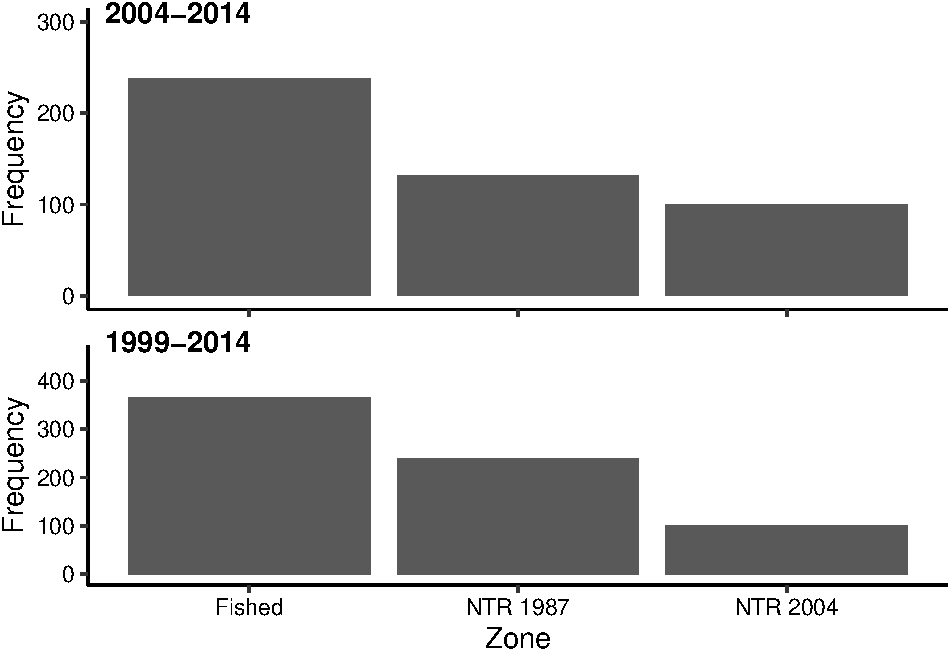
\includegraphics{Mullaney_ENV872_Project_files/figure-latex/Zone Exploratory Plot-1} 

}

\caption{The number of fished zones, no-take zones established in 1987, and no-take zones established in 2004 when data from 1999-2014 are included (bottom) and data from only 2004-2014 are included (top).}\label{fig:Zone Exploratory Plot}
\end{figure}

When examining the frequency of macroalgae and coral percent cover from
1999-2014, macroalgae often has 0\% cover while live coral most
frequently has coverage percentages around 40 (Figure 2); these values
indicate that many of the sampled sites may remain dominated by coral
rather than macroalgae. In looking at the relationship between living
coral and macroalge further, it appears that mean fleshy macroalge
percent cover is negatively correlated with mean living hard coral
percent cover (Figure 3).

\begin{figure}

{\centering 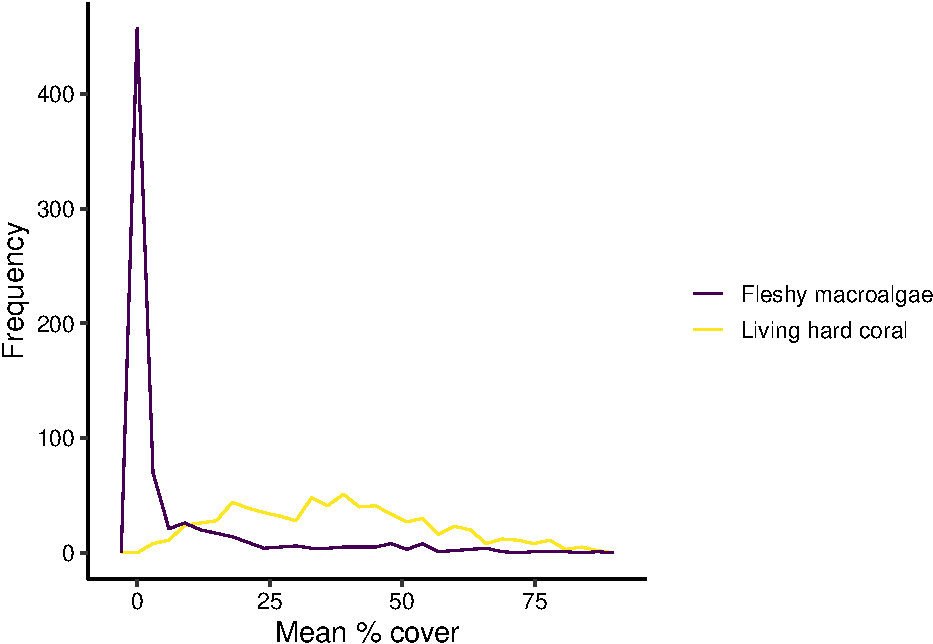
\includegraphics{Mullaney_ENV872_Project_files/figure-latex/Coral Algae Exploratory Plot-1} 

}

\caption{Frequency of fleshy macroalgae percent cover compared to living hard coral percent cover (1999-2014).}\label{fig:Coral Algae Exploratory Plot}
\end{figure}

\begin{figure}

{\centering 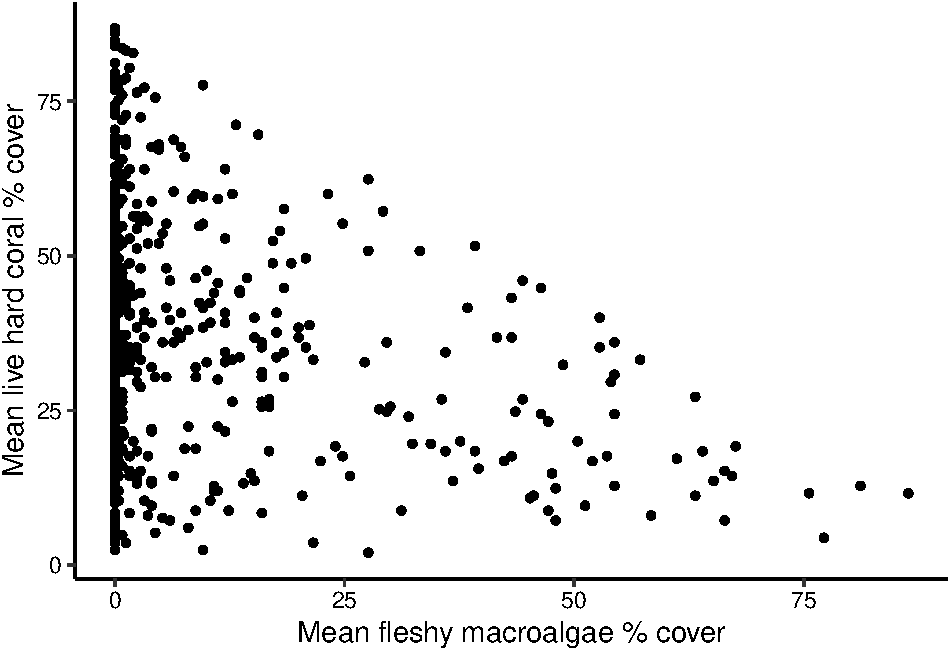
\includegraphics{Mullaney_ENV872_Project_files/figure-latex/Coral Algae Scatter-1} 

}

\caption{Mean fleshy macroalgae percent cover plotted against mean live hard coral percent cover (1999-2014).}\label{fig:Coral Algae Scatter}
\end{figure}

\newpage

In looking at mean fish density and mean percent live hard coral cover
across 2004-2014, it appears as though fish density has the smallest
ranges in 2004 and 2012-2014 (Figure 4). From 2011-2014, coral coverage
has been low compared to 2009, although it has consistently reached
values above 50\% (Figure 4). Coral percent cover seems as though it
could be slightly positively correlated with fish density (Figure 5).

\begin{figure}

{\centering 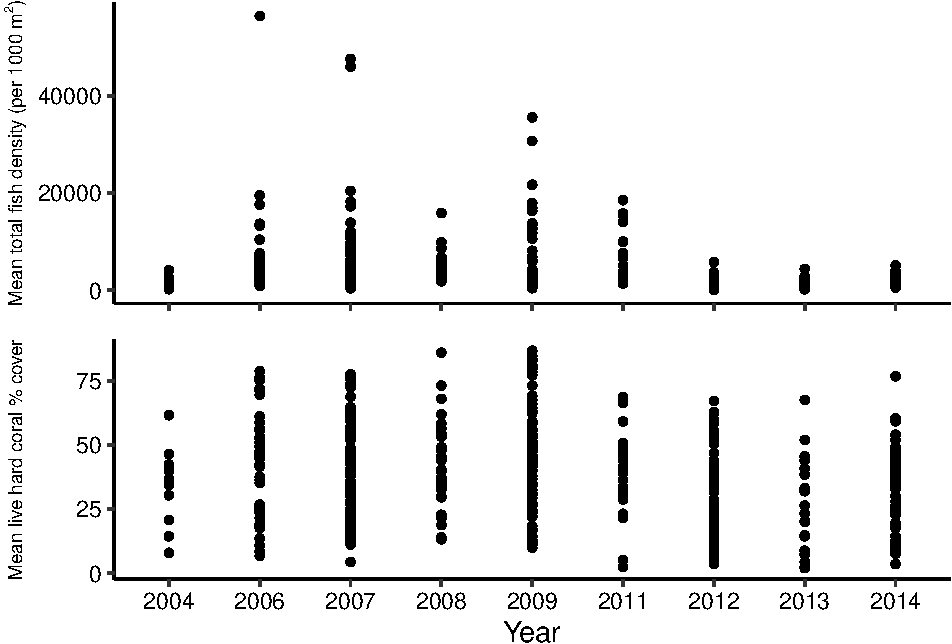
\includegraphics{Mullaney_ENV872_Project_files/figure-latex/Coral Fish Exploratory Plots-1} 

}

\caption{Mean live hard coral percent cover and mean total fish density across 2004, 2006-2009, and 2011-2014.}\label{fig:Coral Fish Exploratory Plots}
\end{figure}

\begin{figure}

{\centering 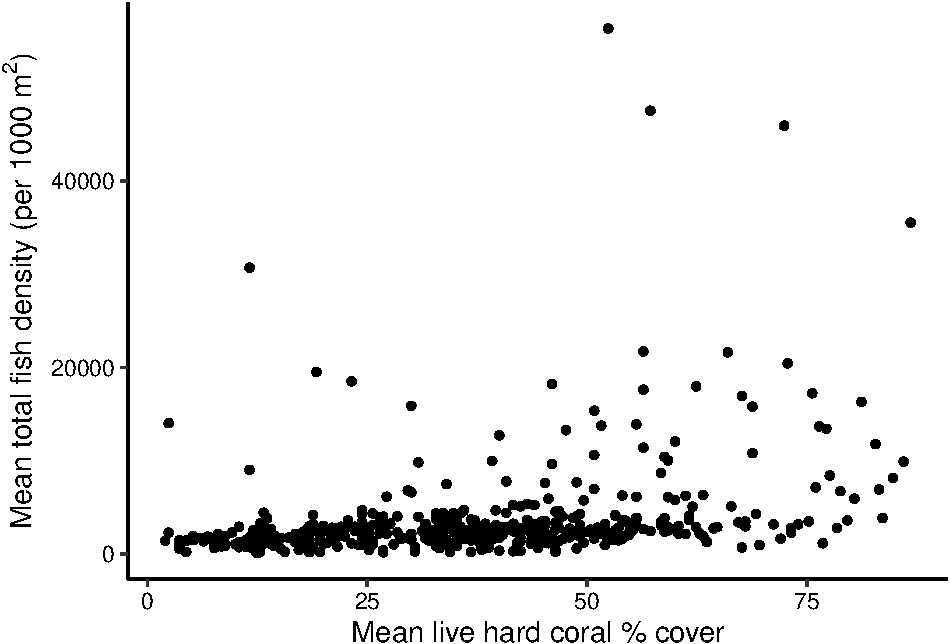
\includegraphics{Mullaney_ENV872_Project_files/figure-latex/Coral Fish Scatter-1} 

}

\caption{Mean live hard coral percent cover plotted against mean total fish density (2004-2014).}\label{fig:Coral Fish Scatter}
\end{figure}

\newpage

\hypertarget{analysis}{%
\section{Analysis}\label{analysis}}

\hypertarget{question-1-what-variables-affect-the-percent-coverage-of-living-hard-coral-on-the-inshore-coral-reefs-of-the-gbrmp}{%
\subsection{Question 1: What variables affect the percent coverage of
living hard coral on the inshore coral reefs of the
GBRMP?}\label{question-1-what-variables-affect-the-percent-coverage-of-living-hard-coral-on-the-inshore-coral-reefs-of-the-gbrmp}}

To determine factors influencing live hard coral cover within the GBRMP,
a mixed-effects analysis of covariance (ANCOVA) model was used. To
account for the random effect of study site and allow extrapolation of
results to potential study sites not included in the data, site was
included as a random effect. The best-fitting model, which was found
using stepwise Akaike information criterion (AIC) analysis, contained
the explanatory variables of year, mean number of grazer fish species,
mean number of corallivore fish species, and mean percentage cover of
fleshy macroalgae. Year, the mean number of grazer fish species, and the
mean percentage cover of fleshy macroalgae significantly decrease the
mean percentage of live hard coral cover, while the mean number of
corallivore fish species significantly increase it (pseudo
R\textsuperscript{2} = 0.8078; Figures 6 \& 7). When all other variables
are held constant, each additional fish included in the mean number of
grazers will decrease mean live hard coral percent cover by 0.0227\% (df
= 358, t = -2.805, p \textless{} 0.05). Similarly, a one unit increase
in the mean macroalgae percent cover will decrease mean live hard coral
percent cover by 0.354\% (df = 358, t = 7.641, p \textless{} 0.0001),
while a one unit increase in the mean number of corallivores will
increase mean live hard coral percent cover by 0.265\% (df = 358, t =
7.812, p \textless{} 0.0001). A post hoc Tukey test was used to evaluate
pairwise relationships of different years and extract groupings based on
these pairwise relationships. Differences in letters between years
indicate statistical differences.

\begin{longtable}[]{@{}ll@{}}
\toprule
Year & Statistical Group\tabularnewline
\midrule
\endhead
2004 & cd\tabularnewline
2006 & bc\tabularnewline
2007 & bc\tabularnewline
2008 & bd\tabularnewline
2009 & d\tabularnewline
2011 & a\tabularnewline
2012 & b\tabularnewline
2013 & a\tabularnewline
2014 & bc\tabularnewline
\bottomrule
\end{longtable}

\begin{figure}

{\centering 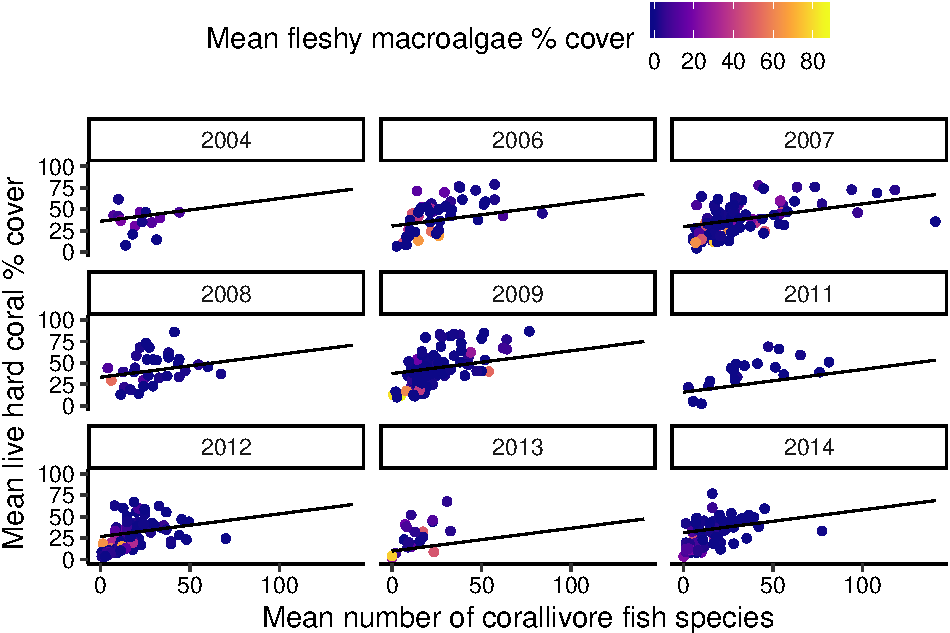
\includegraphics{Mullaney_ENV872_Project_files/figure-latex/Coral Percent Cover Plot (Corallivores)-1} 

}

\caption{Modeled relationship between the mean number of corallivore fish species, the mean percent cover of living hard coral, and the mean percent cover of fleshy macroalgae for 2004, 2006-2009, and 2011-2014. The mean number of grazer fish species was also included in the model (Figure 7). Regression lines are plotted using using the mean number of grazer species and the mean percent cover of fleshy macroalgae for the year corresponding to the facet.}\label{fig:Coral Percent Cover Plot (Corallivores)}
\end{figure}

\begin{figure}

{\centering 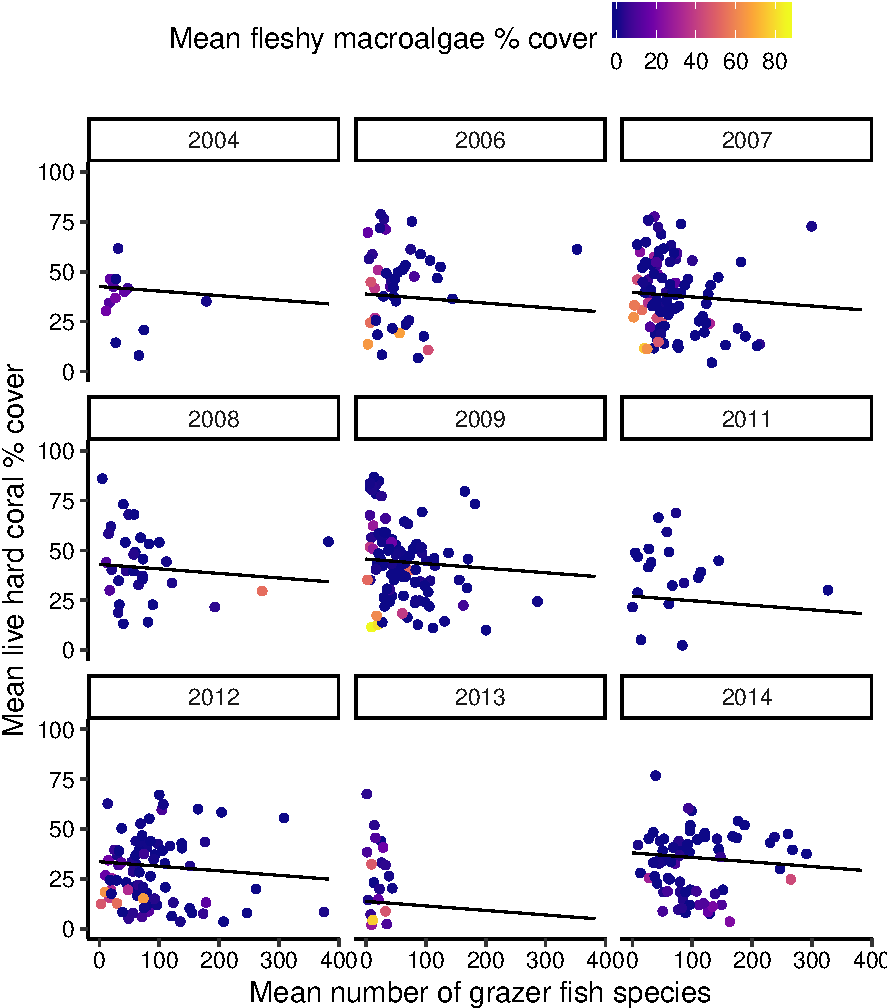
\includegraphics{Mullaney_ENV872_Project_files/figure-latex/Coral Percent Cover Plot (Grazers)-1} 

}

\caption{Modeled relationship between the mean number of grazer fish species, the mean percent cover of living hard coral, and the mean percent cover of fleshy macroalgae for 2004, 2006-2009, and 2011-2014. The mean number of corallivore fish species was also included in the model (Figure 6). Regression lines are plotted using using the mean number of corallivore species and the mean percent cover of fleshy macroalgae for the year corresponding to the facet.}\label{fig:Coral Percent Cover Plot (Grazers)}
\end{figure}

\newpage

\hypertarget{question-2-what-variables-affect-total-fish-density-on-the-inshore-coral-reefs-of-the-gbrmp}{%
\subsection{Question 2: What variables affect total fish density on the
inshore coral reefs of the
GBRMP?}\label{question-2-what-variables-affect-total-fish-density-on-the-inshore-coral-reefs-of-the-gbrmp}}

To determine factors influencing mean total fish density within the
GBRMP, a mixed-effects analysis of covariance (ANCOVA) model was used.
To account for the random effect of study site and allow extrapolation
of results to potential study sites not included in the data, site was
included as a random effect. The best-fitting model, which was found
using stepwise AIC analysis, contained the explanatory variables of year
and mean percentage of live hard coral cover. The mean percentage of
live hard coral cover was found to increase the natural log of mean
total fish density (pseudo R\textsuperscript{2} = 0.8087; Figure 8).
When all other variables are held constant, each additional 1\% of live
hard coral cover will increase the mean total fish density by 1.536\%
(df = 360, t = 7.429, p \textless{} 0.0001). A post hoc Tukey test was
used to evaluate pairwise relationships of different years and extract
groupings based on these pairwise relationships (Figure 8).

\begin{figure}

{\centering 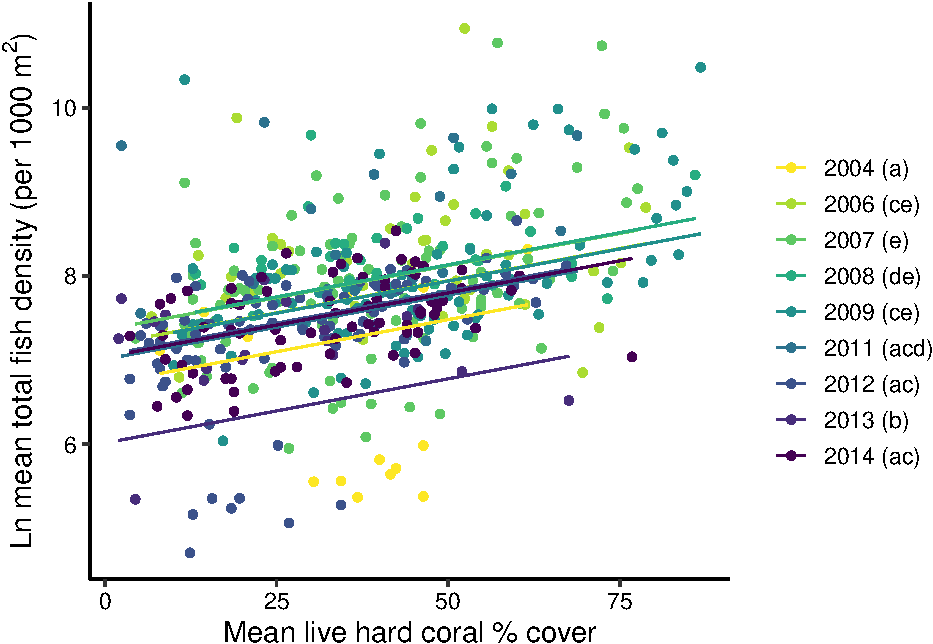
\includegraphics{Mullaney_ENV872_Project_files/figure-latex/Fish Density Plot-1} 

}

\caption{Modeled relationship between the mean percent cover of living hard coral and the natural log of fish density for 2004, 2006-2009, and 2011-2014. Letters indicating pairwise relationships among years are included in the legend; differences in letters between years indicate statistical differences.}\label{fig:Fish Density Plot}
\end{figure}

\hypertarget{question-3-do-no-take-zones-established-in-1987-no-take-zones-established-in-2004-and-fished-zones-have-different-mean-amounts-of-living-hard-coral-cover-total-fish-density-and-fish-species-richness}{%
\subsection{Question 3: Do no-take zones established in 1987, no-take
zones established in 2004, and fished zones have different mean amounts
of living hard coral cover, total fish density, and fish species
richness?}\label{question-3-do-no-take-zones-established-in-1987-no-take-zones-established-in-2004-and-fished-zones-have-different-mean-amounts-of-living-hard-coral-cover-total-fish-density-and-fish-species-richness}}

To determine if mean total fish density, mean fish species richness, and
mean percent coral cover were significantly different among the three
GBRMP zones in the data (no-take since 1987, no-take since 2004, and
fished), three analysis of variance (ANCOVA) models were constructed.
Zone was not found to significantly impact mean percent live coral cover
(F\textsubscript{2,703} = 0.1649, p \textgreater{} 0.1) or mean fish
species richness (F\textsubscript{2,467} = 2.396, p \textgreater{}
0.05). However, zone did significantly affect mean fish species density
(F\textsubscript{2,467} = 6.137, p \textless{} 0.01), with the no-take
zones from 2004 increasing mean fish density by 39.780\% (t = 3.171, p
\textless{} 0.01). A post hoc Tukey test was used to evaluate pairwise
relationships of different zones and extract groupings based on these
pairwise relationships (Figure 9).

\begin{figure}

{\centering 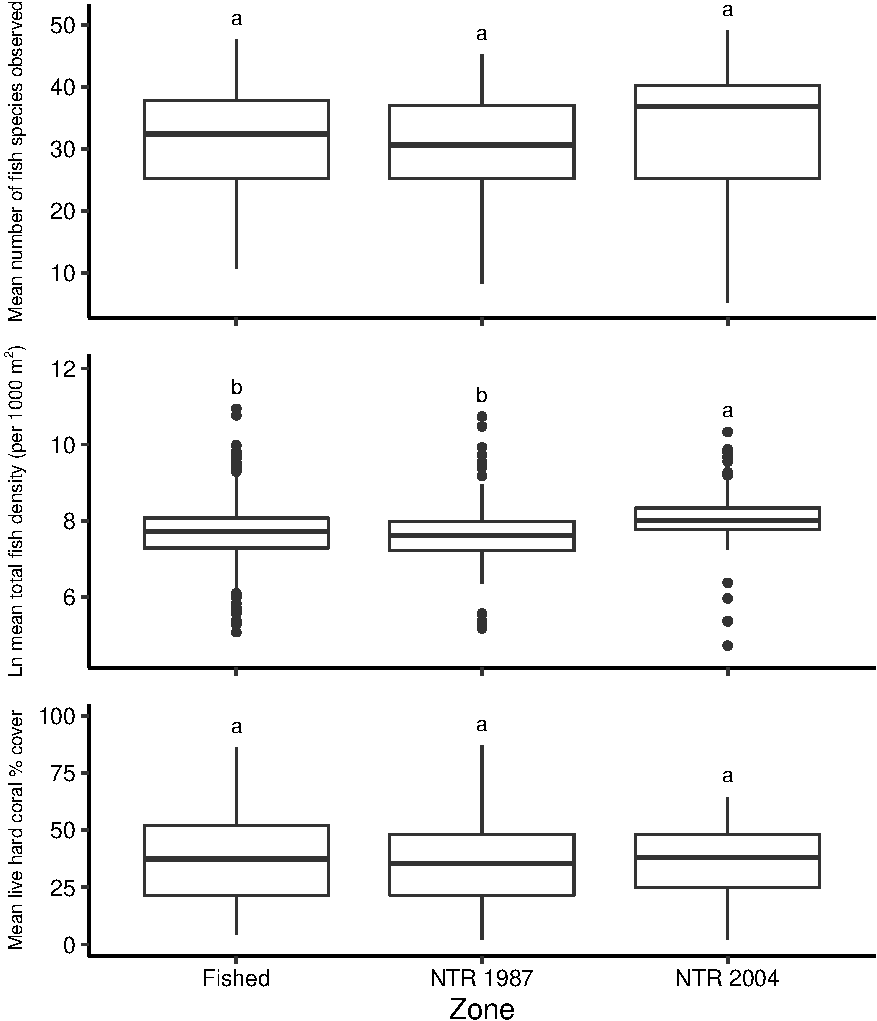
\includegraphics{Mullaney_ENV872_Project_files/figure-latex/Zoning Plots-1} 

}

\caption{Modeled relationship between the GBRMP zone and the mean percent cover of living hard coral from 1999-2014 (bottom), the natural log of fish density (middle) from 2004-2014, and fish species richness from 2004-2014 (top). Letters indicating pairwise relationships among zones are above each bar; differences in letters between zones indicate statistical differences.}\label{fig:Zoning Plots}
\end{figure}
\newpage

\hypertarget{summary-and-conclusions}{%
\section{Summary and Conclusions}\label{summary-and-conclusions}}

Based on these analyses, the percent coverage of living hard coral
depends on several ecological factors -- it is negatively impacted by
greater coverage of macroalgae as well as larger numbers of grazer fish
species, and it is positively impacted by larger numbers of corallivore
fish species. These effects of macroalgae align with previous research,
as macroalgae has been consistently found to compete with corals for
reef space (Bellwood et al.~2004). However, the effects that grazer and
corallivore fish species have on coral coverage are unexpected --
grazers consumemacroalgae and keep its growth under control, while
corallivores inflict damage on coral through consumption. One
explanation for these effects could be that corallivores serve a dual
purpose; perhaps they scrape algae off of coral in the process of
consumption and these benefits overshadow any inflicted harm. It is also
possible that the discovered relationships are actually flipped:
corallivores may be attracted to areas with high amounts of coral
coverage while grazers may be attracted to areas with high amounts of
macroalgae coverage (and thus less coral). Year also affects living hard
coral cover, and while data was not collected at a high enough
resolution to examine clear trends over time, all years that
significantly explained coral coverage decreased it in relation to 2004,
indicating the possibility of a negative trend over time.

Fewer variables significantly impacted the mean total fish density --
based on these analyses, more coral coverage increases fish density, and
each additional 1\% of live hard coral cover will raise the mean total
fish density by 1.536\%. This relationship hints at the profound effects
that coral can have on reef fish communities; an increase coral coverage
results in an even greater rise in fish density.

Surprisingly, zone was not found to significantly affect mean percent
live coral cover or mean fish species richness, despite the
well-researched positive effects of no-take zones relative to fished
zones (Williamson et al.~2004; Lester et al.~2009; Castro-Sanguino et
al.~2017). While the mean fish species density in no-take zones
established in 2004 differs markedly from fished zones -- no-take zones
increase mean fish density by 39.780\% -- it also differed from no-take
zones established in 1987. However, it is possible that management of
no-take zones in the 1980s and 1990s was quite different than management
of these zones today, resulting in unexpected similarities between
no-take zones established in 1987 zones and fished zones. While no
effects of zone on coral coverage were found, it is possible changes in
corals due to zone implementation will only be detectable over a longer
time frame.

These analyses confirmed the negative impacts of macroalgae on reefs as
well as the positive effects of corals on reef fish communities. They
also illuminated areas for future work; more research on the effects of
marine zones and their management practices is necessary to understand
the effects of GBRMP zones on reef and fish assemblages. Continuous
future monitoring is also important to watch for detectable effects of
management practices on coral reef communities.

\newpage

\hypertarget{references}{%
\section{References}\label{references}}

Bellwood DR, Hughes TP, Folke C, Nyström M. 2004. Confronting the coral
reef crisis. Nature. 429(6994):827--833. \url{doi:10.1038/nature02691}.

Castro-Sanguino C, Bozec Y-M, Dempsey A, Samaniego BR, Lubarsky K,
Andrews S, Komyakova V, Ortiz JC, Robbins WD, Renaud PG, et al.~2017.
Detecting conservation benefits of marine reserves on remote reefs of
the northern GBR. PLoS ONE. 12(11):e0186146.

Darling ES, Graham NA, J, Januchowski-hartley FA, Nash KL, Pratchett MS,
Wilson SK. 2017. Relationships between structural complexity, coral
traits, and reef fish assemblages. Coral Reefs; Heidelberg.
36(2):561--575. \url{doi:http://dx.doi.org/10.1007/s00338-017-1539-z}.

FAO, editor. 2018. Meeting the sustainable development goals. Rome (The
state of world fisheries and aquaculture).

Fraser KA, Adams VM, Pressey RL, Pandolfi JM. 2017. Purpose, policy, and
practice: Intent and reality for on-ground management and outcomes of
the Great Barrier Reef Marine Park. Marine Policy. 81:301--311.
\url{doi:10.1016/j.marpol.2017.03.039}.

Lawrey E. 2014. e-Atlas Dataset reporting form.

Lester SE, Halpern BS, Grorud-Colvert K, Lubchenco J, Ruttenberg BI,
Gaines SD, Airamé S, Warner RR. 2009. Biological effects within no-take
marine reserves: a global synthesis. Marine Ecology Progress Series.
384:33--46. \url{doi:10.3354/meps08029}.

Newton K, Côté IM, Pilling GM, Jennings S, Dulvy NK. 2007. Current and
Future Sustainability of Island Coral Reef Fisheries. Current Biology.
17(7):655--658. \url{doi:10.1016/j.cub.2007.02.054}.

Pauly D, Christensen V, Guénette S, Pitcher TJ, Sumaila UR, Walters CJ,
Watson R, Zeller D. 2002. Towards sustainability in world fisheries.
Nature. 418(6898):689--695. \url{doi:10.1038/nature01017}.

Williamson DH, Russ GR, Ayling AM. 2004. No-take marine reserves
increase abundance and biomass of reef fish on inshore fringing reefs of
the Great Barrier Reef. Environmental Conservation. 31(2):149--159.
\url{doi:10.1017/S0376892904001262}.


\end{document}
